% **************************************************
% Clean Thesis
% -- A LaTeX Style for Thesis Documents --
% 
% Copyright (C) 2011-2013 Ricardo Langner
% **************************************************
%
% Readme:
% ----------------------------------------
% *** Clean, Simple, Elegant ***
% "Clean Thesis" is a LaTeX style for thesis documents, developed
% for my diplom thesis (Diplomarbeit). The style can be understood
% as my personal compromise - a typical clean looking scientific
% document combined and polished with minor beautifications.
% 
% The design of this "Clean Thesis" style is inspired
% by user guide documents from Apple Inc.
% 
% Note: If you are looking for an exact and correct style regarding
% typographic rules, please have a look at the "Classic Thesis Style"
% (see http://www.miede.de/index.php?page=classicthesis).
% 
% *** Donation = Postcard ***
% Based on the idea of Andr\'e Miede: If you like the "Clean Thesis"
% style I would be very pleased about a donation in the form of a
% POSTCARD. You can find my address in the file Clean-Thesis.pdf.
% I am going to collect all postcards and exhibit them at the website
% I mentioned.
% 
% *** Idea and Inspiration ***
% The idea of providing my customized style for thesis documents
% passed through my mind while writing my own thesis. Motivated and
% inspired by the superb "Classic Thesis Style"
% (see http://www.miede.de/index.php?page=classicthesis) by Andr\'e Miede
% (thanks to Andr\'e for doing a great job) I decided to collect all
% design and style related functionality in a separate LaTeX style and
% provide this style to other thesis writers.
% 
% 
% License Information:
% ----------------------------------------
% "Clean Thesis" is free software: you can redistribute it and/or modify
% it under the terms of the GNU General Public License as published by
% the Free Software Foundation, either version 3 of the License, or
% (at your option) any later version.
% 
% "Clean Thesis" is distributed in the hope that it will be useful,
% but WITHOUT ANY WARRANTY; without even the implied warranty of
% MERCHANTABILITY or FITNESS FOR A PARTICULAR PURPOSE.  See the
% GNU General Public License for more details.
% 
% You should have received a copy of the GNU General Public License
% along with this program.  If not, see <http://www.gnu.org/licenses/>.
% **************************************************


% **************************************************
% Document Class Definition
% **************************************************
\documentclass[%
	paper=A4,					% paper size --> A4 is default in Germany
	twoside=false,				% onesite or twoside printing
	openright,					% doublepage cleaning ends up right side
	parskip=full,				% spacing value / method for paragraphs
	chapterprefix=true,			% prefix for chapter marks
	11pt,						% font size
	headings=normal,			% size of headings
	bibliography=totoc,			% include bib in toc
	listof=totoc,				% include listof entries in toc
	titlepage=on,				% own page for each title page
	captions=tableabove,		% display table captions above the float env
	draft=false,				% value for draft version
]{scrreprt}%

% **************************************************
% Debug LaTeX Information
% **************************************************
%\listfiles

% **************************************************
% Information and Commands for Reuse
% **************************************************
\newcommand{\thesisTitle}{Final Project CS807}
\newcommand{\thesisName}{Andr\'e Evaristo dos Santos
\\ 
Jhonatan de Souza Oliveira
}
\newcommand{\thesisSubject}{Documentation}
\newcommand{\thesisDate}{March, 2016}
%\newcommand{\thesisVersion}{0.6.8}

%\newcommand{\thesisFirstReviewer}{Jane Doe}
%\newcommand{\thesisFirstReviewerUniversity}{\protect{Clean Thesis Style University}}
%\newcommand{\thesisFirstReviewerDepartment}{Department of Clean Thesis Style}
%
%\newcommand{\thesisSecondReviewer}{John Doe}
%\newcommand{\thesisSecondReviewerUniversity}{\protect{Clean Thesis Style University}}
%\newcommand{\thesisSecondReviewerDepartment}{Department of Clean Thesis Style}

\newcommand{\thesisFirstSupervisor}{Dr. David Gerhard}
%\newcommand{\thesisSecondSupervisor}{John Smith}

\newcommand{\thesisUniversity}{\protect{University of Regina}}
\newcommand{\thesisUniversityDepartment}{Department of Computer Science}
%\newcommand{\thesisUniversityInstitute}{Institut for Clean Thesis Dev}
%\newcommand{\thesisUniversityGroup}{Clean Thesis Group (CTG)}
\newcommand{\thesisUniversityCity}{Regina}
\newcommand{\thesisUniversityStreetAddress}{3737 Wascana Parkway}
\newcommand{\thesisUniversityPostalCode}{S4S 0A2}

% **************************************************
% Load and Configure Packages
% **************************************************
\usepackage[utf8]{inputenc}		% defines file's character encoding
\usepackage[english]{babel} % babel system, adjust the language of the content
\usepackage{marginnote} %margin note
\usepackage{paralist} %inline list
\usepackage{hyperref}
\usepackage[					% clean thesis style
	figuresep=colon,%
	sansserif=false,%
	hangfigurecaption=false,%
	hangsection=true,%
	hangsubsection=true,%
	colorize=full,%
	colortheme=bluemagenta,%
	bibsys=bibtex,
]{cleanthesis}

\hypersetup{					% setup the hyperref-package options
	pdftitle={\thesisTitle},	% 	- title (PDF meta)
	pdfsubject={\thesisSubject},% 	- subject (PDF meta)
	pdfauthor={\thesisName},	% 	- author (PDF meta)
	plainpages=false,			% 	- 
	colorlinks=false,			% 	- colorize links?
	pdfborder={0 0 0},			% 	-
	breaklinks=true,			% 	- allow line break inside links
	bookmarksnumbered=true,		%
	bookmarksopen=true			%
}

% **************************************************
% Document CONTENT
% **************************************************
\begin{document}

% --------------------------
% rename document parts
% --------------------------
%\renewcaptionname{ngerman}{\figurename}{Abb.}
%\renewcaptionname{ngerman}{\tablename}{Tab.}
\renewcaptionname{english}{\figurename}{Fig.}
\renewcaptionname{english}{\tablename}{Tab.}

% --------------------------
% Front matter
% --------------------------
\pagenumbering{roman}			% roman page numbing (invisible for empty page style)
\pagestyle{empty}				% no header or footers
% !TEX root = ../thesis-example.tex
%
% ------------------------------------  --> cover title page
\begin{titlepage}
	\pdfbookmark[0]{Cover}{Cover}
	\flushright
	\hfill
	\vfill
	{\LARGE\thesisTitle} \par
	\rule[5pt]{\textwidth}{.4pt} \par
	{\Large\thesisName}
	\vfill
	\textit{\large\thesisDate} \\
%	Version: \thesisVersion
\end{titlepage}


% ------------------------------------  --> main title page
\begin{titlepage}
	\pdfbookmark[0]{Titlepage}{Titlepage}
	\tgherosfont
	\centering
	
%	{\Large \thesisUniversity} \\[4mm]
	
\includegraphics[width=6cm]{img/logo_uofr_black} \\[2mm]
	\textsf{\thesisUniversityDepartment} \\
%	\textsf{\thesisUniversityInstitute} \\
%	\textsf{\thesisUniversityGroup} \\
	
	\vfill
	{\LARGE \color{ctcolormain}\textbf{\thesisTitle} \\[10mm]}
	{\Large \thesisName} \\
	
	\vfill
%	\begin{minipage}[t]{.27\textwidth}
%		\raggedleft
%		\textit{1. Reviewer}
%	\end{minipage}
%	\hspace*{15pt}
%	\begin{minipage}[t]{.65\textwidth}
%		{\Large \thesisFirstReviewer} \\
%	  	{\small \thesisFirstReviewerDepartment} \\[-1mm]
%		{\small \thesisFirstReviewerUniversity}
%	\end{minipage} \\[5mm]
%	\begin{minipage}[t]{.27\textwidth}
%		\raggedleft
%		\textit{2. Reviewer}
%	\end{minipage}
%	\hspace*{15pt}
%	\begin{minipage}[t]{.65\textwidth}
%		{\Large \thesisSecondReviewer} \\
%	  	{\small \thesisSecondReviewerDepartment} \\[-1mm]
%		{\small \thesisSecondReviewerUniversity}
%	\end{minipage} \\[10mm]
%	\begin{minipage}[t]{.27\textwidth}
%		\raggedleft
%		\textit{Supervisors}
%	\end{minipage}
%	\hspace*{15pt}
%	\begin{minipage}[t]{.65\textwidth}
%		\thesisFirstSupervisor\ and \thesisSecondSupervisor
%	\end{minipage} \\[10mm]
	
	\thesisDate \\
	
\end{titlepage}


% ------------------------------------  --> lower title back for single page layout
\hfill
\vfill
\small
\textbf{\thesisName} \\
\textit{\thesisTitle} \\
\thesisDate \\
%Reviewers: \thesisFirstReviewer\ and \thesisSecondReviewer \\
Instructor: \thesisFirstSupervisor\
%and \thesisSecondSupervisor
\\[1.5em]
\textbf{\thesisUniversity} \\
%\textit{\thesisUniversityGroup} \\
%\thesisUniversityInstitute \\
\thesisUniversityDepartment \\
\thesisUniversityStreetAddress \\
\thesisUniversityPostalCode \thesisUniversityCity
		% INCLUDE: all titlepages
\cleardoublepage

\pagestyle{plain}				% display just page numbers
% !TEX root = Clean-Thesis.tex
%
\pdfbookmark[0]{Abstract}{Abstract}
\chapter*{Abstract}
\label{sec:abstract}
\vspace*{-10mm}

[TODO]
		% INCLUDE: the abstracts (english and german)
\cleardoublepage
%
%% !TEX root = ../thesis-example.tex
%
\pdfbookmark[0]{Acknowledgement}{Acknowledgement}
\chapter*{Acknowledgement}
\label{sec:acknowledgement}
\vspace*{-10mm}

\Blindtext[2][2]
 % INCLUDE: acknowledgement
%\cleardoublepage
%
\setcounter{tocdepth}{2}		% define depth of toc
\tableofcontents				% display table of contents
\cleardoublepage

% --------------------------
% Body matter
% --------------------------
\pagenumbering{arabic}			% arabic page numbering
\setcounter{page}{1}			% set page counter
\pagestyle{maincontentstyle} 	% fancy header and footer

% !TEX root = ../thesis-example.tex
%
\chapter{Introduction}
\label{sec:intro}

\cleanchapterquote{You can’t do better design with a computer, but you can speed up your work enormously.}{Wim Crouwel}{(Graphic designer and typographer)}

\Blindtext[2][2]

\section{Postcards: My Address}
\label{sec:intro:address}

\textbf{Ricardo Langner} \\
Alfred-Schrapel-Str. 7 \\
01307 Dresden \\
Germany


\section{Motivation and Problem Statement}
\label{sec:intro:motivation}

\Blindtext[3][1]

\section{Results}
\label{sec:intro:results}

\Blindtext[1][2]

\section{Thesis Structure}
\label{sec:intro:structure}

\textbf{Chapter \ref{sec:related}} \\[0.2em]
\blindtext

\textbf{Chapter \ref{sec:system}} \\[0.2em]
\blindtext

\textbf{Chapter \ref{sec:concepts}} \\[0.2em]
\blindtext

\textbf{Chapter \ref{sec:concepts}} \\[0.2em]
\blindtext

\textbf{Chapter \ref{sec:conclusion}} \\[0.2em]
\blindtext
 % INCLUDE: introduction
\chapter{Background}
\label{sec:background}

\reversemarginpar

We review [TODO].

%\marginnote{\tiny BAYESIAN NETWORK}

\section{Bayesian Networks}
\label{sec:baysian_networks}


 % INCLUDE: related work
\chapter{Darwin Library}
\label{sec:darwin_lib}

Darwin is a simple library written in Python for BN modeling and inference.
The main purpose of the library is teaching BNs and quick prototyping or testing small networks.
In order to achieve these goals, the library has a simplistic approach of implementation, using native Python data structure and light usage of object oriented programming.
The structure of Darwin is basically divided into two categories: potentials and graph manipulations.
The features are also split into two main categories: inference and modeling tools.
Later, in this section, we also present a guide for getting started using Darwin.

\section{Structure}
\label{sec:system:sec1}

In order to work with BNs, Darwin has two main set of implementations: potential and graph manipulations.
These two categories form individually or together the tree structure of the library as presented in Figure \ref{fig:tree_darwin}.

\begin{figure}[hbt]
    \begin{center}
        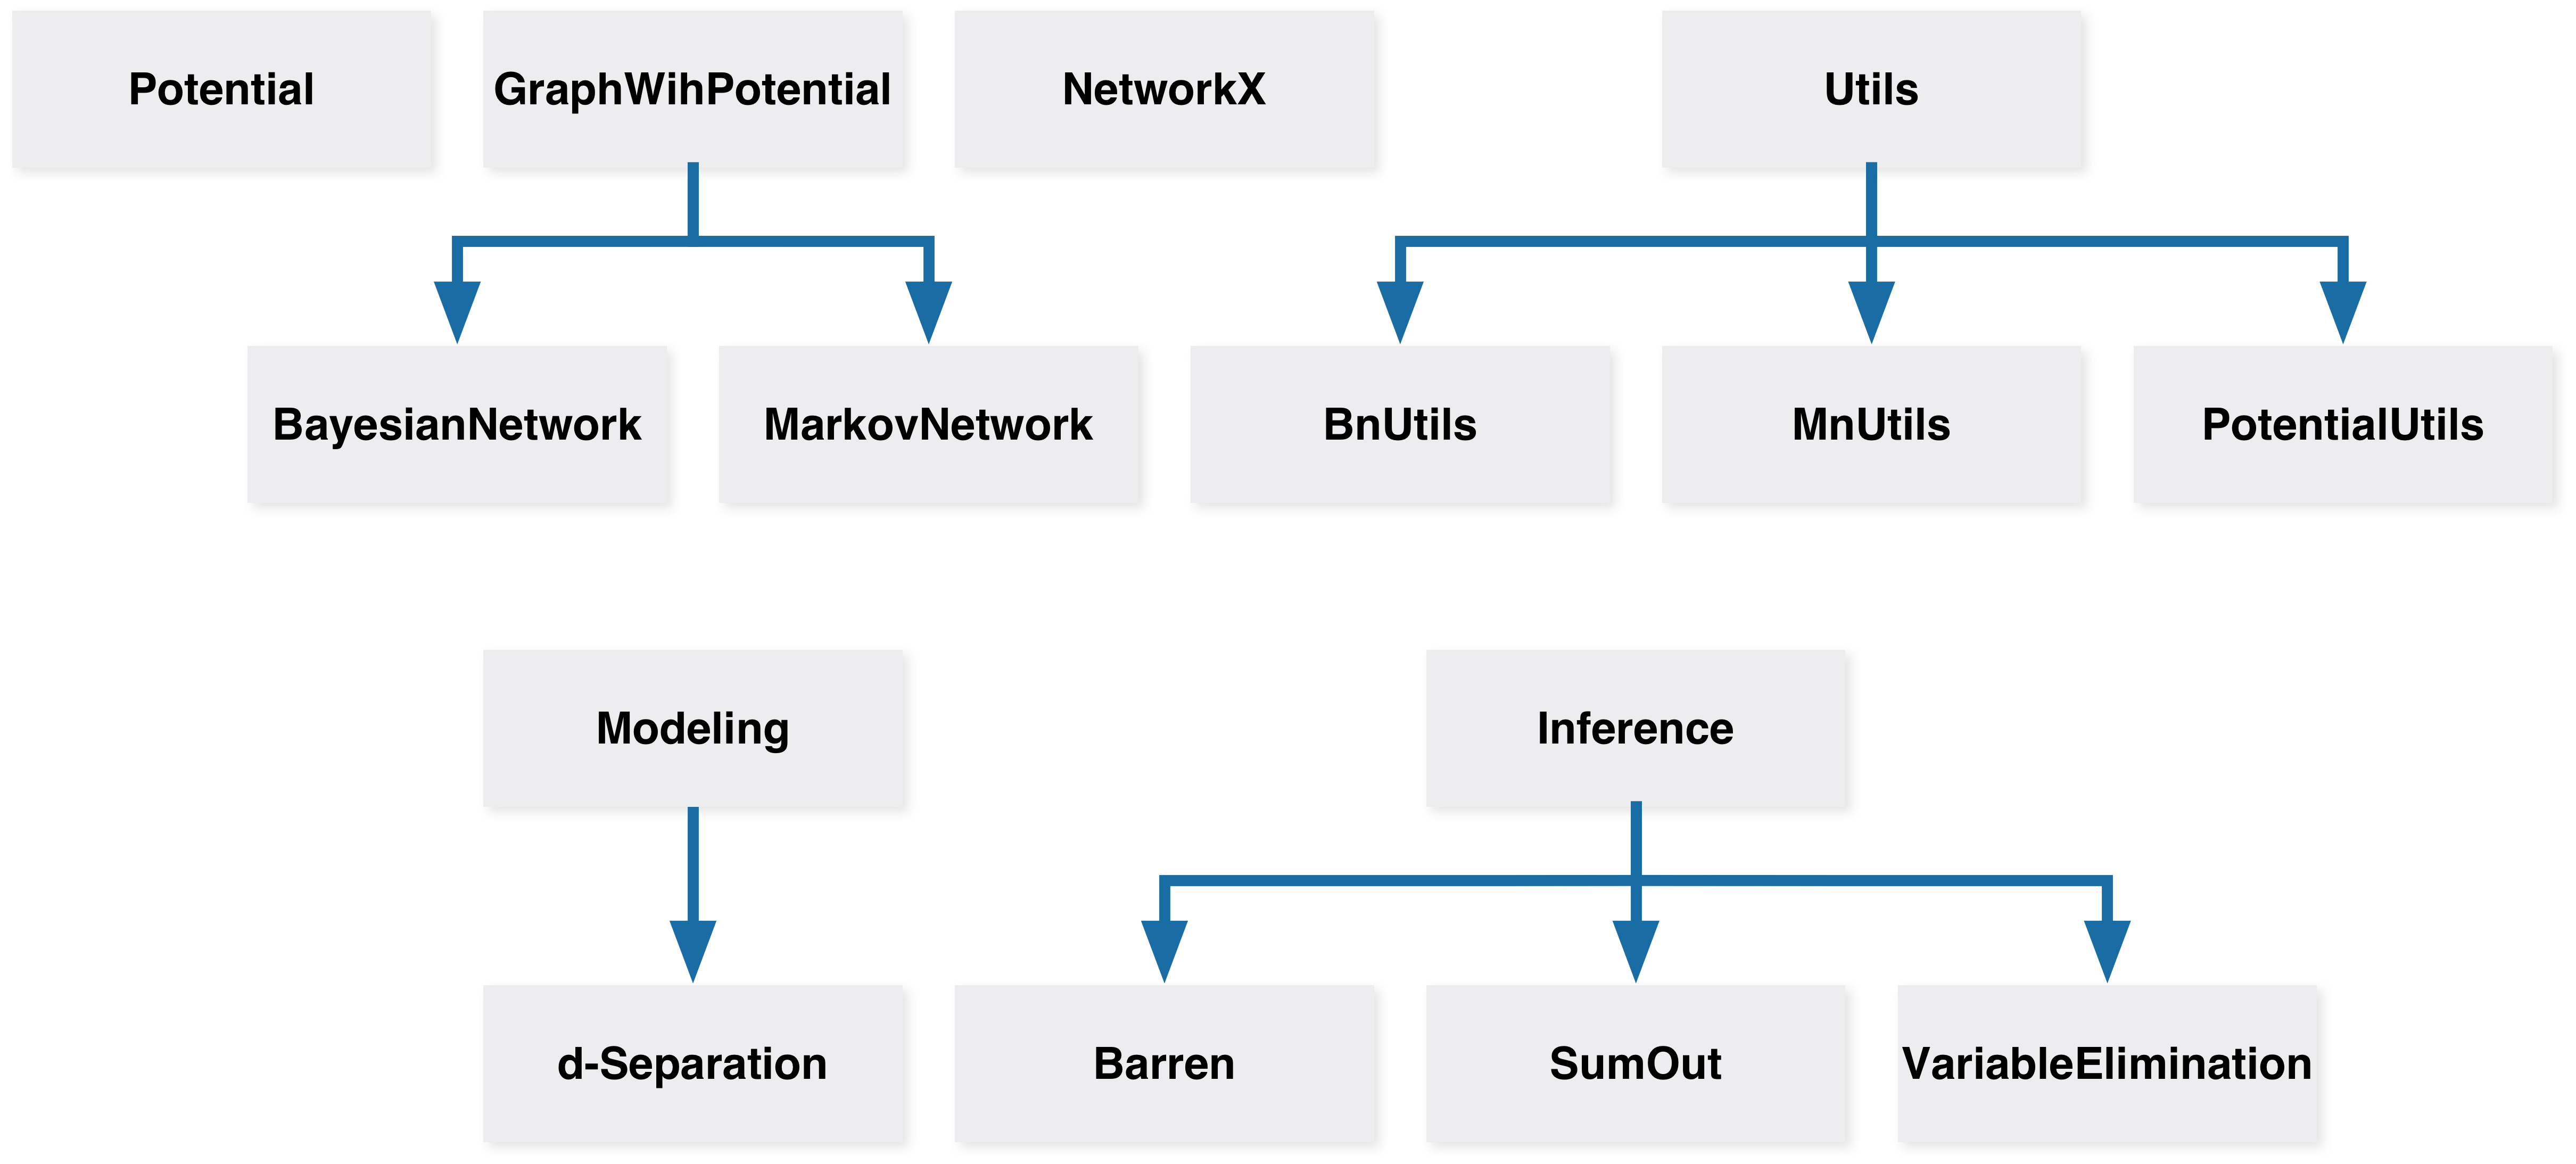
\includegraphics[width=\textwidth]{img/structure_darwin}
    \end{center}
    \caption{Three structure of Darwin.}
    \label{fig:tree_darwin}
\end{figure}

At the root, the class \emph{Potential} is a data structure for modeling a probability table.
The \emph{NetworkX} \cite{hagberg-2008-exploring} is set of data structures for graph manipulation and is also included at the root of the library.
Similarly, \emph{GraphWithPotential} is a class which basically maps nodes in a graph with a set of potentials, besides providing manipulations on the graph and the potentials on it.
\emph{BayesianNetwork} is a class that inherits from \emph{GraphWithPotential} but maps only one potential per node.
This data structure is used for modeling a BN.
In the same way, the class \emph{MarkovNetwork} entirely inherits the behaviour and properties of \emph{GraphWithPotential}, therefore it can be used for MN modeling.

The \emph{Utils} branch is formed by a set of standalone functions which implement core procedures for the other classes.
Mainly, these functions are defined by numerical operations on lists of probabilities.
One advantage of having those implementations as standalone functions is that future optimized code can be included or modified without disturbing the other classes, since the other classes only makes a function call to those utilities functions.
Basically, there are three main utilities: \emph{BnUtils}, \emph{MnUtils}, and \emph{PotentialUtils}.
The BnUtils has a set of functions for BN manipulations and operations, such as moralization, triangulization, join tree construction, among others.
In MnUtils, we have utilities for MN propagation such as finding an optimal path for propagating in a tree.
Lastly, PotentialUtils is formed by a set of procedures for numerical operations such as multiplication, division and marginalization of tables.
All potential manipulations in PotentialUtils is implemented according to the efficient implementation proposed in \cite{koll09}.

In the \emph{Modeling} brach, there is an implementation of d-Separation as proposed in Algorithm 3.1 of \cite{koll09}.
While in the branch \emph{Inference} there are few data structures useful for exact inference in BNs.
The \emph{Barren} function is used for identifying barren potentials in factorizations.
\emph{SumOut} is a function which systematically removes a set of variables from a factorization by multiplying potentials with the variables and them marginalizing the variables out.
The class \emph{VariableElimination} implements the exact inference algorithm VE as originally proposed by \cite{zhan94}.
Finally, the \emph{Test} branch has a set of unit tests which assure the correct functioning of core functions in the whole library.

\section{Features}
\label{sec:system:sec2}

Here, we highlight some feature of the library.
In general, the features are tools to facilitate the use of Darwin in teaching and prototyping of small system.
The library is not intended for fast inference, neither high accuracy.
Therefore, all numerical operations are implemented using native Python code, instead of high performance libraries such as \emph{numpy} \cite{van2011numpy}.
The graph manipulations are done by an external library called \emph{NetworkX}, a robust and well known library with high performance and large set of tools.

For modeling, Darwin has the testing of d-Separation implemented using a reachability algorithm.
Also, the library has built in tools for converting a BN into a MN, including the join tree construction by moralization, triangulization and the assignment of potentials.
The triangulization step, specifically, has implemented 4 different heuristics, the same as implemented in \emph{PgmPy} \footnote{http://pgmpy.org}.

For inference, the library provides a basic function for eliminating variables in a factorization, called \emph{SumOut}.
But for faster inference, it is recommended to use the VE implementation which absorb evidence, removes barren and independent by evidence potentials, perform inference by summing out non relevant variables and, finally, normalize the final result.

\section{Usage}
\label{sec:system:sec3}

In order to get started with Darwin, we now present a quick overview of the most common classes and functions.
The main classes are \emph{Potential}, \emph{GraphWithPotential}, \emph{BayesianNetwork}, and \emph{MarkovNetwork}.

The Potential class is defined by the given arguments: \emph{variables} which is a list with strings, \emph{cardinalities} corresponding to the variables which is a list with integers in the same order than the variables, probabilities \emph{values} in a list with floating numbers, \emph{left hand side} which is a list with the variables in the LHS of the potential, and similarly the \emph{right hand side} is defined.
For example, considering a CPT $P(a|b)$ with binary variables and probability values 0.4, 0.5, 0.6, 0.5, we can use Darwin to represent this potential as:
\begin{verbatim}
    Potential(["a", "b"], [2, 2], [0.4, 0.5, 0.6, 0.5], ["b"], ["a"])
\end{verbatim}

The GraphWithPotential class contains basically a list with potentials, a graph defined using NetworkX, and a dictionary mapping nodes in the graph to a list of potentials.
After declaring a GraphWithPotential, the user can add potentials to a node using the \emph{add\_potential} method.
For example, the following code creates a graph with two nodes $\{a\}$ and $\{a,b\}$ and assign $P(a)$ to $\{a\}$ and $P(b|a)$ to $\{a,b\}$ in a GraphWithPotential.
\begin{verbatim}
    p1 = Potential(["a"], [2], [0.2, 0.8], ["a"], [])
    p2 = Potential(["a", "b"], [2, 2], [0.4, 0.5, 0.6, 0.5], ["b"], ["a"])
    
    G = networkx.Graph()
    G.add_nodes(["a", "ab"])
    
    GwP = GraphWithPotential()
    GwP.add_potential("a", p1)
    GwP.add_potential("ab", p2)
\end{verbatim}

The MarkovNetwork inherits from GraphWithPotential, therefore modeling a MN is simply using the GraphWithPotential like in the code above.
In the same way, modeling a BN uses the BayesianNetwork class which also inherits from GraphWithPotential.
The difference for a BN is that only one potential is assigned at one node and the graph used is a DAG.
For instance, the code above can be used to declare a BN with two nodes $a \rightarrow ab$ just by changing the definition of $G$ to the below code, which is a directed graph.
\begin{verbatim}
    G = networkx.DiGraph()
    G.add_edge("a", "ab")
\end{verbatim}
	% INCLUDE: system
\chapter{Darwinian Network Library}
\label{sec:dn_lib}

\section{Structure}
\label{sec:system:sec1}

The DN library is a simple extension of Darwin, also intended for teaching and prototyping purposes.
Basically, the library inherits the potential manipulation tools from Darwin, ignoring the graphical manipulation ones.
From there, DN library builds the analysis of set of potentials, which forms a DN by definition.
The structure of the library is mainly formed by two classes: \emph{Population} and \emph{DarwinianNetwork}.

The Population class inherits directly from Potential's class in Darwin.
But here, few keywords are override in order to adapt the language for DNs.
For instance, the left and right hand side of the arguments in a Potential are called combative and docile in a Population.
Moreover, a Population have the methods merge and replicate which internally calls multiply (or divide) and marginalize from Potential.
Deciding where it is a division or multiplication is handled internally by the merge method.

DarwinianNetworks is defined with a set of Populations.
This data structure basically offers common methods for set manipulations, for instance, inserting and removing Populations.
Here, the set of populations are stored in an array, in order to allow the multiset populations as defined in DNs.

\section{Features}
\label{sec:system:sec2}

Few features are present in DN library in order to guarantee a smooth use for teaching and prototyping.
Now, we highlight there features of the library: keyword usage, initialization of parameters and drawing of data structure.

When instantiating a Population, the user can use keywords for the combative and docile arguments.
In this way, the user does not need to remember the ordering of the arguments, but only their names.
For example, defining a population $p(a,b)$ can be defined with the below code by using keywords ``combative'' and ``docile'':
\begin{verbatim}
    Population(combative=["a"],docile=["b"])
\end{verbatim}

Also for simplifying usage, the library has standard initialization of internal parameters.
That is, if the user does not pass all the required arguments, the DN library initialize them correctly when possible with standard values.
For example, in the above code the cardinalities of variables ``a'' and ``b'' are set to 2 and the 4 probabilities values are randomly generated between 0 and 1.

Finally, the DN library has a set of procedures for drawing Populations and DarwinianNetworks whenever the user calls them.
Those tools are built using the \emph{matplotlib} \cite{Hunter:2007} library for Python and is the only requirement for the drawings.
If the user wants to see how a population looks like, the user can define the Population and then calls the \emph{draw\_population} function as illustrate below:
\begin{verbatim}
    p = Population(combative=["d"],docile=["f", "b"])
    draw_population(p)
\end{verbatim}
These commands will create a drawing of a population as illustrated in Figure \ref{fig:drawing_pop}.

\begin{figure}[hbt]
    \begin{center}
        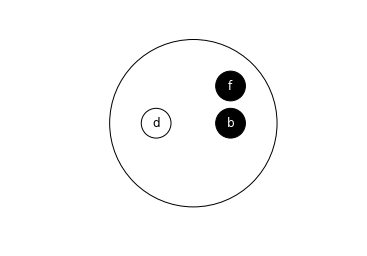
\includegraphics[width=0.6\textwidth]{img/drawing_population.png}
    \end{center}
    \caption{Drawing of population $p(d,fb)$ created by the DN library.}
    \label{fig:drawing_pop}
\end{figure}

The same idea works for a whole DN.
After defining a DarwinianNetwork, the user can call \emph{draw\_dn} passing the DN object.
Figure \ref{fig:drawing_dn} shows one example of the drawing of a DN as generated by the DN library.

\begin{figure}[hbt]
    \begin{center}
        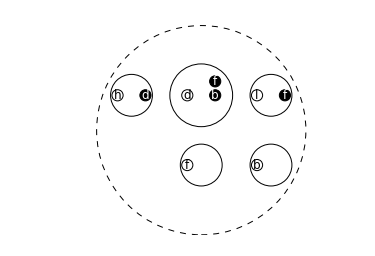
\includegraphics[width=0.6\textwidth]{img/drawing_dn.png}
    \end{center}
    \caption{Drawing of the DN $\{p(h,d), p(l,f), p(f), p(b), p(d,fb)\}$ created by the DN library.}
    \label{fig:drawing_dn}
\end{figure}

\section{Usage}
\label{sec:system:sec3}

The use of the two main classes in DN library is introduced now.
The Population class is defined exactly like a Potential, since it inherits from that class.
But the left and right hand side argument names are replaced by combative and docile, respectively.
Two methods are also exposed for quick references: combative and docile, which returns the respective informations for that Population.
A helper method called \emph{from\_potential} is also available in order to convert a Potential object to a Population one.
Moreover, merge receives another Population as argument, while replicate receives a list of variables which will be marginalized from the Population.

The DarwinianNetwork class has a list member where all the Populations are hold.
The methods \emph{add\_population} and \emph{delete\_population} are used for adding and deleting Population, respectively, from the list of Populations
This class has no constructor and the list of Populations is used to simulate the multi-set definition of DNs.
 % INCLUDE: concepts
\chapter{Conclusion}
\label{sec:conclusion}

We proposed Darwinian Network Library as new framework for modeling and inference in DNs.
DN library is a implementation of the basic operations for adaptation and evolution in DNs.
It is implemented with the Python programming language and the basic data structures are provided by Darwin library.
%It provides salient features as test unity and a tutorials with IPython Notebook.
The main advantage of the DN library is to apply novel ideas and techniques of DNs.
DN library also is great for teaching, quick prototyping with DNs and testing.


DN library is based upon the novel library Darwin, a Python framework for BN modeling and inference.
Darwin library has two main categories called potentials and graph manipulations.
The former is a data structure for modeling a probability table.
The latter maps nodes in the graph to a list of potentials.
Together they form a reliable structure to reason on BNs.

We have established in Chapter \ref{sec:dn_lib} features of DN library given the manipulation tools from Darwin.
We have shown that DN library is an intuitive framework for working with DNs.
For instance, to build a set of potentials, one can simply utilize the class \emph{Population}.
Intuitively, with objects \emph{Population} together we can obtain a class \emph{DarwinianNetwork}.

Another salient feature is the set of procedures for drawing Populations and DarwinianNetworks.
It allows the user to see how looks like a population that has just been created - or even the entire DN!


This project proposes the implementation of a DN library.
In summary, we have stablished four main advantages of using DN library:
\begin{inparaenum}[(i)]
\item due its simple approach given the Python implementation, it has an expressive language that facilitate its usage;
\item it has interactive visual tools to compute and draw DNs, enabling users to better interact with the library;
\item it is a great tool for learning and its operations are sound given the unit tests;
\item and all source code is available free online on \emph{GitHub} through the webpage:
\end{inparaenum}
\begin{center}
\url{https://github.com/Darwinian-Networks}
\end{center}
With DN library, DNs can be applied as the simple and yet remarkably robust tool they are, allowing users to simplify reasoning with BNs.
 % INCLUDE: conclusion
\cleardoublepage

% --------------------------
% Back matter
% --------------------------
%{%


%\setstretch{1.1}
%\renewcommand{\bibfont}{\normalfont\small}
%\setlength{\biblabelsep}{0pt}
%\setlength{\bibitemsep}{0.5\baselineskip plus 0.5\baselineskip}
%\nocite{*}
%\printbibliography[nottype=online]
%\printbibliography[heading=subbibliography,title={Webseiten},type=online,prefixnumbers={@}]
%}
%\cleardoublepage

\bibliographystyle{splncs03}
\bibliography{references}


%\listoffigures
%\cleardoublepage
%
%\listoftables
%\cleardoublepage
%
%% !TEX root = ../thesis-example.tex
%
\pagestyle{empty}
\hfill
\vfill
\pdfbookmark[0]{Colophon}{Colophon}
\section*{Colophon}

This thesis was typeset with \LaTeXe.
It uses the \textit{Clean Thesis} style developed by Ricardo Langner.
The design of the \textit{Clean Thesis} style is inspired by user guide documents from Apple Inc.

Download the \textit{Clean Thesis} style at \url{http://cleanthesis.der-ric.de/}.

%\cleardoublepage
%
%% !TEX root = ../thesis-example.tex
%
%************************************************
% Declaration
%************************************************
\pdfbookmark[0]{Declaration}{Declaration}
\chapter*{Declaration}
\label{sec:declaration}
\thispagestyle{empty}

You can put your declaration here, to declare that you have completed your work solely and only with the help of the references you mentioned.

\bigskip

\noindent\textit{\thesisUniversityCity, \thesisDate}

\smallskip

\begin{flushright}
	\begin{minipage}{5cm}
		\rule{\textwidth}{1pt}
		\centering\thesisName
	\end{minipage}
\end{flushright}

%*****************************************
%*****************************************

%\clearpage
%\newpage
%\mbox{}

% **************************************************
% End of Document CONTENT
% **************************************************
\end{document}
